\documentclass[letterpaper,10pt]{article}

\usepackage{enumitem}
\usepackage{titling}
\usepackage{listings,listings-rust}
\usepackage{url}
\usepackage{soul}
\usepackage{hyperref}
\usepackage{setspace}
\usepackage{subfig}
\usepackage{sectsty}
\usepackage{pdfpages}
\usepackage{colortbl}
\usepackage{multirow}
\usepackage{multicol}
\usepackage{relsize}
\usepackage{amsmath}
\usepackage{wasysym}
\usepackage{fancyvrb}
\usepackage[yyyymmdd]{datetime}
\usepackage{amsmath,amssymb,amsthm,graphicx,xspace}
\usepackage[titlenotnumbered,noend,noline]{algorithm2e}
\usepackage[compact]{titlesec}
\usepackage{XCharter}
\usepackage[T1]{fontenc}
\usepackage[scaled]{beramono}
\usepackage[normalem]{ulem}
\usepackage{booktabs}
\usepackage{tikz}
\usetikzlibrary{arrows.meta,automata,shapes,trees,matrix,chains,scopes,positioning,calc,decorations.pathreplacing}
\tikzstyle{block} = [rectangle, draw, fill=blue!20, 
    text width=2.5em, text centered, rounded corners, minimum height=2em]
\tikzstyle{bw} = [rectangle, draw, fill=blue!20, 
    text width=4em, text centered, rounded corners, minimum height=2em]

\definecolor{namerow}{cmyk}{.40,.40,.40,.40}
\definecolor{namecol}{cmyk}{.40,.40,.40,.40}
\renewcommand{\dateseparator}{-}

\let\LaTeXtitle\title
\renewcommand{\title}[1]{\LaTeXtitle{\textsf{#1}}}

\lstset{basicstyle=\footnotesize\ttfamily,breaklines=true}

\newcommand{\CPP}{C\nolinebreak\hspace{-.05em}\raisebox{.4ex}{\tiny\bf +}\nolinebreak\hspace{-.10em}\raisebox{.4ex}{\tiny\bf +}}
\def\CPP{{C\nolinebreak[4]\hspace{-.05em}\raisebox{.4ex}{\tiny\bf ++}}}

\newcommand{\handout}[5]{
  \noindent
  \begin{center}
  \framebox{
    \vbox{
      \hbox to 5.78in { {\bf ECE459: Programming for Performance } \hfill #2 }
      \vspace{4mm}
      \hbox to 5.78in { {\Large \hfill #4  \hfill} }
      \vspace{2mm}
      \hbox to 5.78in { {\em #3 \hfill \today} }
    }
  }
  \end{center}
  \vspace*{4mm}
}

\newcommand{\lecture}[3]{\handout{#1}{#2}{#3}{Lecture#1}}
\newcommand{\tuple}[1]{\ensuremath{\left\langle #1 \right\rangle}\xspace}

\addtolength{\oddsidemargin}{-1.000in}
\addtolength{\evensidemargin}{-0.500in}
\addtolength{\textwidth}{2.0in}
\addtolength{\topmargin}{-1.000in}
\addtolength{\textheight}{1.75in}
\addtolength{\parskip}{\baselineskip}
\setlength{\parindent}{0in}
\renewcommand{\baselinestretch}{1.5}
\newcommand{\term}{Winter 2020}

\singlespace


\begin{document}

\lecture{5 --- Concurrency and Parallelism}{\term}{Jeff Zarnett, based on original by Patrick Lam}

\section*{Concurrency and Parallelism}
Concurrency and parallelism both give up the
total ordering between instructions in a sequential program, for
different purposes.

\paragraph{Concurrency.} We'll refer to the use of threads for
structuring programs as concurrency. Here, we're not aiming
for increased performance. Instead, we're trying to write the program
in a natural way. Concurrency makes sense as a model for distributed
systems, or systems where multiple components interact, with no ordering
between these components, like graphical user interfaces.

\paragraph{Parallelism.} We're studying parallelism in this class, where
we try to do multiple things at the same time in an attempt to increase
throughput. Concurrent programs may be easier to parallelize.

\subsection*{Limits to parallelization}
I mentioned briefly in Lecture 1 that programs often have a sequential
part and a parallel part. We'll quantify this observation today
and discuss its consequences.

\paragraph{Scalable Algorithms.} 
Remember from ECE~250/CS~138 that we often care about the worst case run-time performance of the algorithm. An algorithm that's $O(n^{3})$ scales so much worse than one that's $O(n)$ that it's not even funny. Trying to do an insertion sort on a small array is fine (actually... recommended); doing it on a huge array is madness. Choosing a good algorithm is very important if we want it to scale. 

\begin{center}
	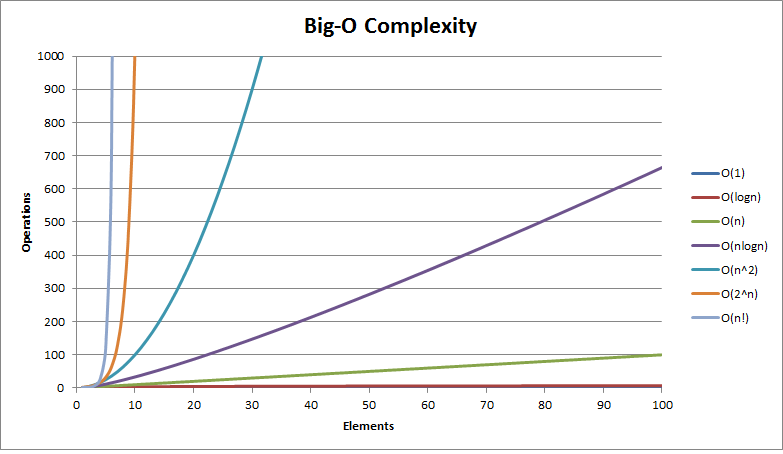
\includegraphics[width=0.75\textwidth]{images/big-o-complexity}\\
	Big-O Complexity comparison from ~\cite{bigocheatsheet}
\end{center}


\paragraph{Amdahl's Law.} One classic model of parallel execution
is Amdahl's Law. In 1967, Gene Amdahl argued that improvements in
processor design for single processors would be more effective than
designing multi-processor systems. Here's the argument. Let's say that
you are trying to run a task which has a serial part, taking fraction 
$S$, and a parallelizable part, taking fraction $P = 1-S$. Define $T_s$
to be the total 
amount of time needed on a single-processor system.
Now, moving to a parallel system with $N$ processors, the parallel
time $T_p$ is instead:
\[ T_p = T_s \cdot (S + \frac{P}{N}). \]
{\bf As $N$ increases, $T_p$ is dominated by $S$, limiting potential
speedup.}

We can restate this law in terms of speedup, which is the 
original time $T_s$ divided by the sped-up time $T_p$:
\[ \mbox{speedup} = \frac{T_s}{T_p} = \frac{1}{S+P/N}. \]
Replacing $S$ with $(1-P)$, we get:
\[ \mbox{speedup} = \frac{1}{(1-P)+P/N}, \]
and
\[ \mbox{max speedup} = \frac{1}{(1-P)}, \]
since $\frac{P}{N} \rightarrow 0$.

\paragraph{Plugging in numbers.} If $P = 1$, then we can indeed get good
scaling; running on an $N$-processor machine will give you a speedup
of $N$. Unfortunately, usually $P < 1$.  Let's see what happens.

\begin{center}
\begin{tabular}{r|r}
$P$ & speedup ($N=18$) \\ \hline
1 & 18 \\
0.99 & $\sim$ 15 \\
0.95 & $\sim$ 10 \\
0.5 & $\sim$ 2
\end{tabular}
\end{center}
Graphically, we have something like this:
\begin{center}
  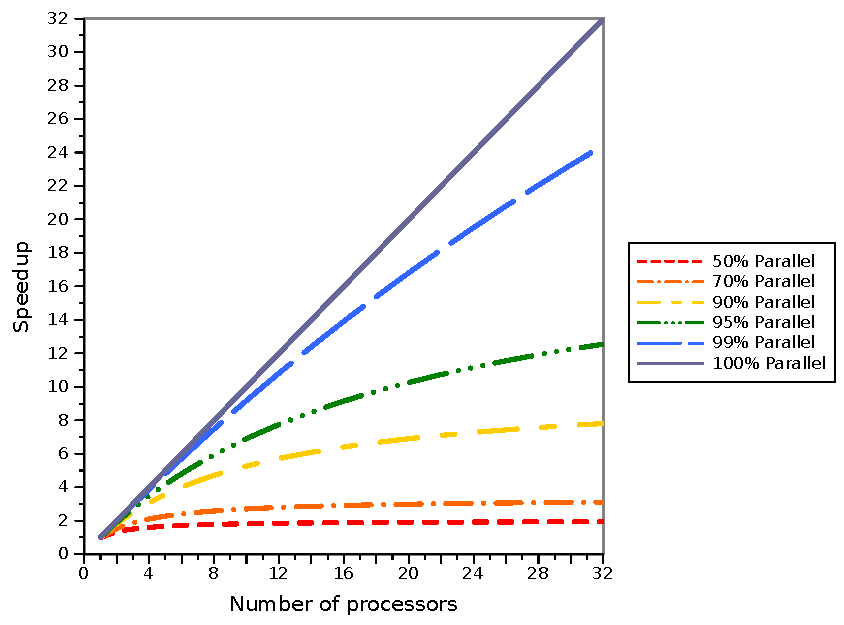
\includegraphics[width=0.5\textwidth]{images/parallel-scaling}
\end{center}


Amdahl's Law tells you how many cores you can hope to leverage in an
execution given a fixed problem size, if you can estimate $P$.

Let us consider an example from~\cite{mte241}: Suppose we have a task that can be executed in 5~s and this task contains a loop that can be parallelized. Let us also say initialization and recombination code in this routine requires 400~ms. So with one processor executing, it would take about 4.6~s to execute the loop. If we split it up and execute on two processors it will take about 2.3~s to execute the loop. Add to that the setup and cleanup time of 0.4~s and we get a total time of 2.7~s. Completing the task in 2.7~s rather than 5~s represents a speedup of about~46\%. Applying the formula, we get the following run times:

\begin{center}
	\begin{tabular}{l|l}
	\textbf{Processors} & \textbf{Run Time (s)} \\ \hline
	1 & 5\\
	2 & 2.7\\
	4 & 1.55\\
	8 & 0.975\\
	16 & 0.6875 \\
	32 & 0.54375 \\
	64 & 0.471875 \\
	128 & 0.4359375\\
	\end{tabular}
\end{center}

   \paragraph{Empirically estimating parallel speedup $P$.}
Assuming that you know things that are actually really hard to know, here's a formula for estimating speedup. You don't have to commit it to memory:
  \[P_{\mbox{\scriptsize estimated}} = \frac{\frac{1}{\mbox{\em speedup}}-1}{\frac{1}{N}-1}.\]

It's just an estimation, but you can use it to guess the fraction of parallel code, given $N$ and the speedup. You can then use $P_{\mbox{\scriptsize estimated}}$ to predict speedup for a different number of processors.

\paragraph{Consequences of Amdahl's Law.}
For over 30 years, most performance gains did indeed come from
increasing single-processor performance. The main reason that we're
here today is that, as we saw last time,
single-processor performance gains have hit the wall.

By the way, note that we didn't talk about the cost of synchronization
between threads here. That can drag the performance down even more.

\paragraph{Amdahl's Assumptions.}
Despite Amdahl's pessimism, we still all have multicore computers today.
Why is that? Amdahl's Law assumes that:
\begin{itemize}[noitemsep]
    \item problem size is fixed (read on);
    \item the program, or the underlying implementation, behaves the same on 1 processor as on $N$ processors; and
    \item that we can accurately measure runtimes---i.e. that overheads don't matter.
\end{itemize}

% replace Amdahl's law with how branch predictors work
%% \paragraph{Generalizing Amdahl's Law.} We made a simplification,
%% which was that programs only have one parallel part and one serial part.
%% Of course, this is not true. The program may have many parts,
%% each of which we can tune to a different degree.

%% Let's generalize Amdahl's Law:

%% \begin{itemize}
%% \item  $f_1, f_2, \ldots, f_n$: fraction of time in part $n$
%% \item  $S_{f_1}, S_{f_n}, \ldots, S_{f_n}$: speedup for part $n$
%% \end{itemize}

%% Then,
%% \[\mbox{\em speedup} = \frac{1}{\frac{f_1}{S_{f_1}} + \frac{f_2}{S_{f_2}} + \ldots +
%%     \frac{f_n}{S_{f_n}}}.\]

%% \paragraph{Example.} Consider a program with 4 parts in the following scenario:

%% \begin{center}
%%     \begin{tabular}{r|r|r|r}
%%     \multicolumn{2}{l}{} & \multicolumn{2}{|c}{Speedup} \\
%%     Part & Fraction of Runtime & Option 1 & Option 2\\
%%     \hline
%%     1 & 0.55 & 1  & 2\\
%%     2 & 0.25 & 5  & 1\\
%%     3 & 0.15 & 3  & 1\\
%%     4 & 0.05  & 10 & 1\\
%%     \end{tabular}
%% \end{center}

%%     (Note: these speedups don't have to be speedups from parallelization.)
    
%%   We can implement either Option 1 or Option 2. 
%%   Which option is better?

%%   ``Plug and chug'' the numbers:
%% \begin{itemize}
%% \item  {\bf Option 1.}

%%   \[ \mbox{\em speedup} = \frac{1}{0.55 + \frac{0.25}{5} + \frac{0.15}{3} + \frac{0.05}{5}}
%%     = 1.53  \]

%% \item  {\bf Option 2.}

%%   \[\mbox{\em speedup} = \frac{1}{\frac{0.55}{2} + 0.45} = 1.38 \hspace*{5.5em}\]
%% \end{itemize}

\subsection*{A more optimistic point of view}
In 1988, John Gustafson pointed
out\footnote{\url{http://www.scl.ameslab.gov/Publications/Gus/AmdahlsLaw/Amdahls.html}}
that Amdahl's Law only applies to fixed-size problems, but that the
point of computers is to deal with bigger and bigger problems.

In particular, you might vary the input size, or the grid resolution,
number of timesteps, etc. When running the software, then, you might
need to hold the running time constant, not the problem size: you're
willing to wait, say, 10 hours for your task to finish, but not 500
hours. So you can change the question to: how big a problem can you
run in 10 hours?

According to Gustafson, scaling up the problem tends to increase the
amount of work in the parallel part of the code, while leaving the
serial part alone. As long as the algorithm is linear, it is possible
to handle linearly larger problems with a linearly larger number of
processors.

Of course, Gustafson's Law works when there is some ``problem-size''
knob you can crank up.  As a practical example, observe Google, which
deals with huge datasets.


\section*{Software Design Issues}


\paragraph{Locking.}
Think back to a concurrency course and the discussion of locking. We'll be coming back to this subject before too long. But for now, suffice it to say, that the more locks and locking we need, the less scalable the code is going to be. You may think of the lock as a resource and the more threads or processes that are looking to acquire that lock, the more ``resource contention'' we have, and the more waiting and coordination are going to be necessary.

\paragraph{Memory Allocators.}
Assuming we're not working with an embedded system where all memory is statically allocated in advance, there will be dynamic memory allocation. The memory allocator is often centralized and may support only one thread allocating or deallocating at a time. This means it does not necessarily scale very well. There are, however, some techniques for dynamic memory allocation that allow these things to work in parallel.

\paragraph{Pools of Worker Threads.}
We'll talk about threads shortly. At first, one might imagine manually starting the necessary threads. But that's not the only way. We can have a pool of workers. Then the application just submits units of work, and then on the other side these units of work are allocated to workers. The number of workers will scale based on the available hardware. This is neat as a programming practice: as the application developer we don't care quite so much about the underlying hardware. Let the operating system decide how many workers there should be, to figure out the optimal way to process the units of work.

\section*{Processes and Threads} Let's review the
difference between a process and a thread. A \emph{process} is an
instance of a computer program that contains program code and its own
address space, stack, registers, and resources (file handles, etc).  A
\emph{thread} usually belongs to a process. The most important point
is that it shares an address space with its parent process, hence
variables and code as well as resources. Each thread has its own~\cite{osi}:
\begin{enumerate}
	\item Thread execution state (like process state: running, ready, blocked...).
	\item Saved thread context when not running.
	\item Execution stack.
	\item Local variables.
	\item Access to the memory and resources of the process (shared with all threads in that process).
\end{enumerate}

Or, to represent this visually:

\begin{center}
	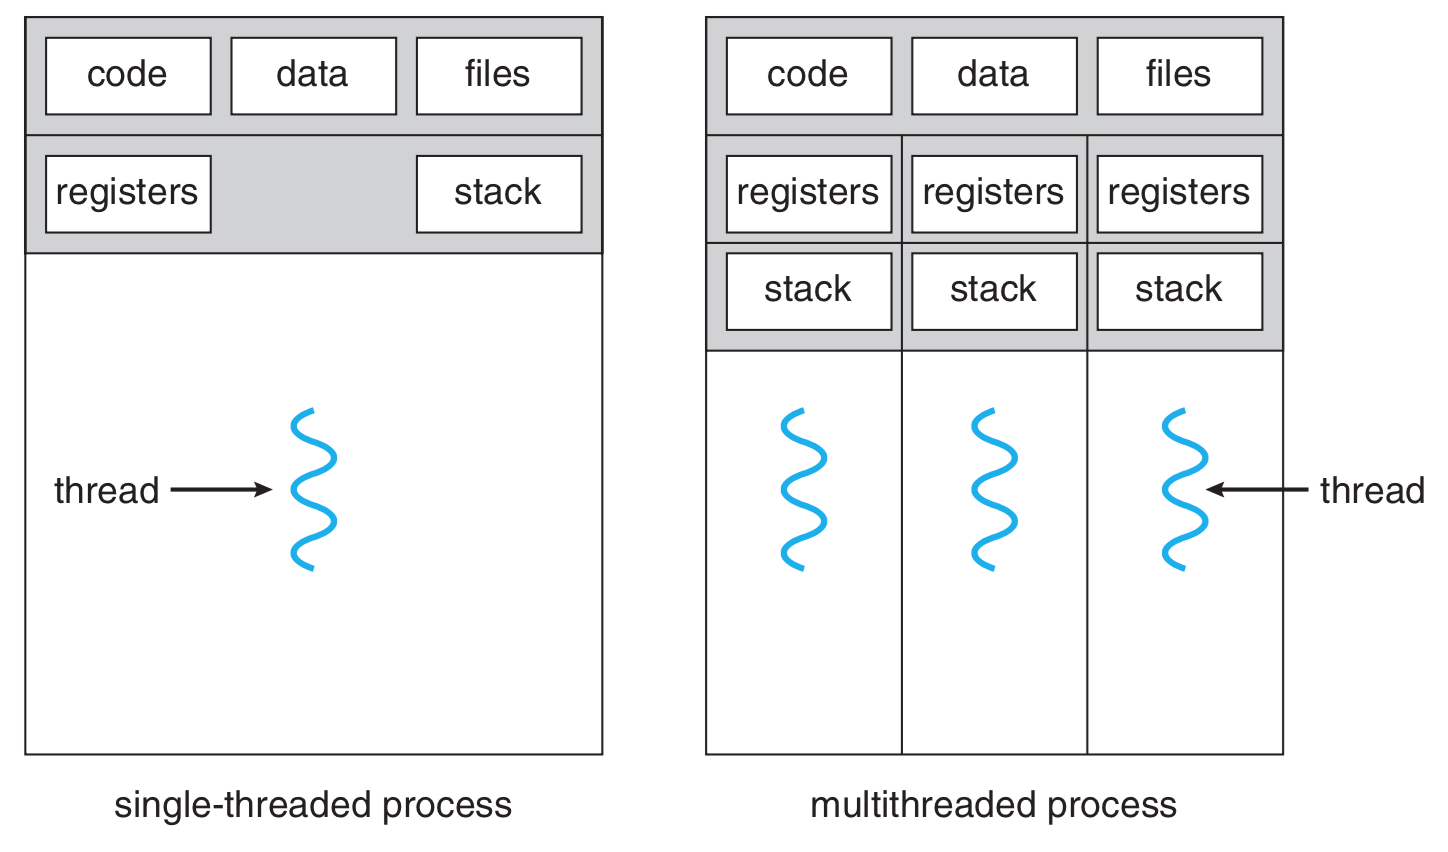
\includegraphics[width=0.6\textwidth]{images/mthread2.png}\\
	A single threaded and a multithreaded process compared side-by-side~\cite{osc}.
\end{center}

All the threads of a process share the state and resources of the process. If one thread opens a file, other threads in that process can also access that file.

The way programs are written now, there are few, if any, that are not in some way multithreaded. One common way of dividing up the program into threads is to separate the user interface from a time-consuming action.

Consider a file-transfer program. If the user interface and upload method share a thread, once a file upload has started, the user will not be able to use the UI anymore (and Windows will put the dreaded ``(Not Responding)'' at the end of its dialog title), even to click the button that cancels the upload. For some reason, users hate that. 

We have two options for how to alleviate this problem: when an upload is ready to start, we can call \texttt{fork} and create a new process to do the upload, or we can spawn a new thread. In either case, the newly created entity will handle the upload of the file. The UI remains responsive, because the UI thread is not waiting for the upload method to complete.

\subsection*{Motivation for Threads}

Why choose threads rather than creating a new process? The primary, but not sole, motivation is performance:
\begin{enumerate}
	\item Creating a new thread is much faster than creating a new process. In fact, thread creation is on the order of ten times faster~\cite{machThreads}.
	\item Terminating and cleaning up a thread is faster than terminating and cleaning up a process.
	\item It takes less time to switch between two threads within the same process (because less data needs to be stored/restored). In Solaris, for example, switching between processes is about five times slower than switching between threads~\cite{osc}.
	\item Because threads share the same memory space, for two threads to communicate, they do not have to use any of the IPC mechanisms; they can just communicate directly.
	\item As in the file transfer program, use of threads allows the program to be responsive even when a part of the program is blocked.
\end{enumerate}

This last advantage, background work, is one of four common examples of the uses of threads in a general purpose operating system~\cite{insideOS2}:
\begin{enumerate}
	\item \textbf{Foreground and Background Work:} as already examined, the ability to run something in the background to keep the program responsive.
	\item \textbf{Asynchronous processing}: for example, to protect against power failure or a crash, a word processor may write the document data in main memory to disk periodically. This can be done as a background task so it does not disrupt the user's workflow.
	\item \textbf{Speed of Execution:} a multithreaded program can get more done in the same amount of time. Just as the OS can run a different program when the executing program gets blocked (say, on a disk read), if one thread is blocked, another thread may execute.
	\item \textbf{Modular Structure:} a program that does several different things may be given structure through threads.
\end{enumerate}

There are some drawbacks, however: there is no protection between threads in the same process. So, one thread can easily mess with the memory being used by another thread. This once again brings us to the subject of co-ordination, which will follow the discussion of threads.

Also, if any thread encounters an error (such as a division by zero or Segmentation Fault), the whole process might be terminated by the operating system. If the program has multiple processes for different parts, then the other processes will not be affected. But, if the program has multiple threads and they all share the same process, then any thread encountering an error might bring all of them to a halt. (That's why Google Chrome chose to use separate processes for each tab.)



You can find another explanation of processes versus threads here:
\begin{center}
  \url{https://www.purplealienplanet.com/node/50}
\end{center}

\paragraph{Threads and CPUs.} In your operating systems class,
you've seen implementations of threads (``lightweight processes'').
We'll call these threads \emph{software threads}, and we'll program
with them throughout the class. Each software thread corresponds to a
stream of instructions that the processor executes. On a old-school
single-core, single-processor machine, the operating system
multiplexes the CPU resources to execute multiple threads
concurrently; however, only one thread runs at a time on the single
CPU.

On the other hand, a modern chip contains a number of \emph{hardware
threads}, which correspond to the virtual CPUs. These are sometimes
known as \emph{strands}. The operating system still needs to 
multiplex the software threads onto the hardware threads, but now has
more than one hardware thread to schedule work onto.



\paragraph{Implementing (or Simulating) Hardware Threads.} 
There are a number of ways to implement multiple software threads; for
instance, the simplest possible implementation, {\bf kernel-level
threading} (or 1:1 model) dedicates one core to each thread. The kernel schedules threads
on different processors. (Note that kernel involvement will always be required to
take advantage of a multicore system). This model is used by Win32, as well as
POSIX threads for Windows and Linux. The 1:1 model allows concurrency and parallelism.

Alternately, we could make one core execute multiple threads. In the
{\bf user-level threading}, or N:1, model, the single core would keep
multiple contexts and could 1) switch every 100 cycles; 2) switch
every cycle; 3) fetch one instruction from each thread each cycle; or
4) switch every time the current thread hits a long-latency event
(cache miss, etc.) This model allows for quick context switches, but
does not leverage multiple processors. (Why would you use these?) The N:1 model is used by
GNU Portable Threads.

Finally, it's possible to both use multiple cores and put multiple
threads onto one core, in a {\bf hybrid threading}, or M:N, model. Here, we map $M$ application threads to $N$ kernel threads. This
is a compromise between the previous two models, which both allows
quick context switches and the use of multiple processors. However, it
requires increased complexity; the library provides scheduling
services, which may not coordinate well with kernel, and increases
likelihood of priority inversion (which you've seen in Operating
Systems).  This method is used by modern Windows threads.


\section*{Choose Your Pain}
The first design decision that you need to solve when parallelizing programs
is whether you should use threads or processes.

  \begin{itemize}
    \item Threads are basically light-weight processes which piggy-back on
          processes' address space.
  \end{itemize}

Traditionally (pre-Linux 2.6) you had to use {\tt
  fork}~(for~processes) and {\tt clone} (for threads). But {\tt clone}
is not POSIX compliant, and its man page says that it's
Linux-specific---FreeBSD uses {\tt rfork()}. (POSIX is the standard
for Unix-like operating systems).

\paragraph{When processes are better.} {\tt fork} is safer and more secure than threads.

  \begin{enumerate}
    \item Each process has its own virtual address space:
      \begin{itemize}
        \item Memory pages are not copied, they are copy-on-write. Therefore, processes use less memory than you would expect.
      \end{itemize}
    \item Buffer overruns or other security holes do not expose other~processes.
    \item If a process crashes, the others can continue.
  \end{enumerate}

{\bf Example:} In the Chrome browser, each tab is a separate
process. Scott McCloud explained this:
\url{http://www.scottmccloud.com/googlechrome/}.

\paragraph{When threads are better.} Threads are easier and faster.

  \begin{enumerate}
    \item Interprocess communication (IPC) is more complicated and slower than interthread
          communication; must use operating system utilities (pipes, semaphores, shared
              memory, etc) instead of thread library (or just memory reads and writes).
    \item Processes have much higher startup, shutdown, and synchronization costs than threads.
    \item pthreads fix the issues of {\tt clone} and provide a
          uniform interface for most systems. (You'll work with them in Assignment 1.)
  \end{enumerate}

\paragraph{How to choose?}
  If your application is like this:
  \begin{itemize}
    \item mostly independent tasks, with little or no communication;
    \item task startup and shutdown costs are negligible compared to overall runtime; and
    \item want to be safer against bugs and security holes,
  \end{itemize}
then processes are the way to go. If it's the opposite of this, then use threads.

For performance reasons, along with ease and consistency across systems, we'll use threads. We will describe both pthreads and C++ 11 threads, in particular.

\paragraph{Overhead of Processes vs Threads.} The common wisdom is that processes are
expensive, threads are cheap. Let's verify this with a benchmark on a
laptop (included in the live-coding directory on GitHub) which creates and destroys 50,000 threads:
  \begin{lstlisting}[basicstyle=\scriptsize]
jon@riker examples master % time ./create_fork 
0.18s user 4.14s system 34% cpu 12.484 total
jon@riker examples master % time ./create_pthread 
0.73s user 1.29s system 107% cpu 1.887 total
  \end{lstlisting}

Clearly pthreads incur much lower overhead than {\tt fork}. pthreads
offer a speedup of 6.5 over processes in terms of startup and teardown costs.

%\paragraph{Live Coding Example.} We can write a program to determine
%whether we are in a user-level threading model vs. the other two models.
%Just start a child thread and make both threads compute. If CPU utilization
%exceeds 100\%, we are not user-level threading. The example I saw in class
%computes $2^{28}$ random numbers to spin the CPU.

%(Is it possible to differentiate hybrid and kernel threading by writing a
%simple program?)




\bibliographystyle{alphaurl}
\bibliography{459}


\end{document}
